\section{The Dynamic Grid}\label{sec:dynamicGrid}
The time variation of the wave speed $c$ leads to various complications in the simulation framework presented above. First of all, a change in $c$ causes a change in $\lambda$ according to Eq. \eqref{eq:compactLambda}, affecting the simulation quality and bandwidth. Secondly, and more importantly, a change in $c$ could result in a change in $N$ through Eq. \eqref{eq:orderOfCalcGrid}. As $N$ directly relates to the number of grid points, this raises questions as to \textit{where} and especially \textit{how} one would add and remove points to the grid according to the now-dynamic wave speed.

We propose a method that allows for a non-integer number of intervals to smoothly change between grid configurations, i.e, the number of grid points. This removes the necessity of the flooring operation in Eqs. \eqref{eq:orderOfCalcGrid} and \eqref{eq:compactLambda}, and consequently satisfies the CFL condition in \eqref{eq:CFL} with equality at all times. Introducing fractional number of intervals $\Nfrac$, where $N = \lfloor \Nfrac\rfloor$, Eq. \eqref{eq:fundamentalFreqCont} can be rewritten in terms of $\Nfrac$ by substituting the calculation of $N$ from \eqref{eq:orderOfCalcGrid} into Eq. \eqref{eq:fundamentalFreqCont} (using $h=ck$) yielding
\begin{equation}\label{eq:fundamentalFreq}
    f_0 = \frac{1}{2\Nfrac k}\quad \text{with}\quad \Nfrac = L/h.
\end{equation}
%\SWcomment[shouldn't $\Nfrac$, $h$, $c$, $M$, $M_w$ all get the $n$ superscript from here onwards?]\SBcomment[Yes! And $f_{0}$ too.] \SWcomment[Alright, I added it to the intro of \ref{sec:proposedMethod} (or do you think from the start of this section already?)]
This shows that if $\lambda = 1$, $\Nfrac$ solely determines the fundamental frequency of the simulation. 

% As mentioned in the previous section, the goal of this paper is to achieve real-time  parameter changes by dynamically changing grid configurations, in order to prevent undesirable behaviour such as a decrease in bandwidth and increase in numerical dispersion. % discussed in Section \ref{sec:quality}. %This section will describe the problems that arise when adding and removing grid points. Afterwards, some iterations done over the course of this project and their drawbacks will be shown, leading up to the final implementation of the dynamic grid. 

% The first questions that need to be answered are ``where to add points?" and ``how to add points?" The problems when doing this range from artifacts or auditory `clicks' in the output sound to ``exploding" systems due to artificial injection of energy. 
% The rest of this section\SBcomment[Which section? Not sure you need this description of the contents. This material almost belongs up in Section 1.] will list the requirements of a method that dynamically changes FDTD grid configurations. %Then, the iterations done over the course of this project will briefly be described, the details of each can be found in Appendix \ref{app:A}. \SWcomment[(I think I might remove the iterations and appendix actually..)] 
% Then, the proposed method will be described in detail and summarised, and finally, some details on its implementation are given. 

% \subsection{Method requirements}\label{sec:methodReq}
% \SBcomment[Do you need a new section for this?]
Ideally, a method that dynamically changes the grid size of a FDS should
\begin{enumerate}[label={r\arabic*.}]
    \item generate an output with a fundamental frequency $f_0$ %described by Eq. \eqref{eq:fundamentalFreq} 
    which is proportional to the wave speed $c$ ($f_0 \propto c$),
    \item allow for a fractional number of intervals $\Nfrac$ to smoothly (without audible artefacts) transition between different grid configurations,% so that no auditory artefacts are present in the output sound,
    \item generate an output containing $ N-1$ modes which are integer multiples of the fundamental ($f_p = f_0 p$ with integer $p$),
    % \item generate an output with $\lfloor N\rfloor-1$ modes corresponding to the number of moving points of the system ($p = [1, \hdots, \allowbreak\lfloor N\rfloor-1]$),
    \item work in real time to have a playable simulation.
\end{enumerate}
These requirements will be used in Section \ref{sec:discussion} to evaluate the proposed method.
%
% The total amount of modes is expected to be equal to $N-1$ corresponding to the total number of moving grid points (points excluding the boundary).
%As the variables $c$, $h$, $\lambda$ and $N$ are now time-varying, a superscript $n$ or $n-1$ is added when necessary. If omitted, a time index $n$ is assumed.

% \subsection{Iterations \SWcomment[(optional section)]}\label{sec:iterations} 
% One method that could be used to go from one grid configuration to the next is full-grid interpolation as described in \cite[Chap. 5]{bilbao2009}. However, this method essentially has a lowpassing effect on the entire system state and can cause `clicks' in the output sound due to the interpolation. A (much) higher sample rate could be used to avoid these issues, but this would render this method impossible to work in real time.

% Another method is to add and remove points at the boundary using an interpolated boundary condition, the possibility of which has been briefly mentioned in \cite[p. 145]{bilbao2009}. If the boundary is fixed through Eq. \eqref{eq:contDirichlet}, the state at this location will always be $0$ and potentially allows for smooth entry and exit of grid points at this location. This method can be seen analogous to tuning a guitar string where string-material enters and leaves the playable part of the string at the nut, the boundary. The interpolated nature of the boundary does allow for a ``fractional" $N$ as described in Section \ref{sec:dynamicParams} and has a fundamental frequency calculated using \eqref{eq:fundamentalFreq}. %removing the flooring operation in Eq. \eqref{eq:compactLambda} and always satisfying the CFL condition with equality. \SWcomment[This has the added feature that $L/h$ in Eq. \eqref{eq:numberOfIntervals} is an integer and the flooring operation can be ignored. Substituting Eq. \eqref{eq:numberOfIntervals} into Eq. \eqref{eq:fundamentalFreqCont} (using Eq. \eqref{eq:stabilityCond} satisfied with equality) yields
%\begin{equation}%\label{eq:fundamentalFreq}
%     f_0 = \frac{1}{2Nk}\ ,
% \end{equation}
% which shows that if $\lambda = 1$, $N$, which is now not necessarily an integer, solely decides the fundamental frequency of the simulation.] 
% Although informal testing shows that adding points to the grid can happen smoothly, removing points smoothly is more challenging. This is due to the fact that the grid point at the boundary will be moving right before it is removed and its displacement needs to (somehow) smoothly be reduced to 0 to satisfy the fixed boundary condition in Eq. \eqref{eq:contDirichlet}. %\SWcomment[$\leftarrow$ if simply supported condition is mentioned here] Even though the $\delta_{xx}u$ part of this condition can be easily satisfied, the $u=0$ part can not.

\subsection{Proposed Method}\label{sec:proposedMethod}
% This section introduces the proposed method to dynamically and smoothly change the grid of FDSs to account for dynamic parameter changes. %To avoid the issues of adding and removing points at the boundary due to boundary conditions, they can be added or removed along the grid instead. \SWcomment[$\leftarrow$ Revise sentence if iterations are removed] For the sake of simplicity, the location is chosen to be the center of the system. %\SWcomment[At the end of this section, the location exhibiting the best behaviour will be shown.] 
In the following, the location of a grid point (in m from the left boundary) $q_l$ at time index $n$ is denoted by $x_{q_l}^n$. %\SBcomment[OK, here, why the switch from grid index $l$ to grid index $i$?] \SWcomment[because $i$ is not a spatial index, but a grid point (with a spatial index). So $x_i$ means ``the x-location of grid point $i$''. I thought it would avoid confusion, but if you think it's better to use $l$, please let me know :)]
Furthermore, some variables are now time dependent as indicated by superscript $n$. These are $c^n$, $h^n$, $\Nfrac^n$, $N^n$ and $f_0^n$.

\subsubsection{System Setup}\label{sec:systSetup}
Consider two grid functions, $u_\lu^n$ and $w_\lw^n$ defined over discrete domains $\lu \in \{0, \hdots, M^n\}$ and $\lw \in \{0, \hdots, M_w^n\}$ respectively with integers $M^n = \lceil 0.5N^n\rceil $ with $\lceil \cdot \rceil$ denoting the ceiling operation and $M_w^n = \lfloor 0.5N^n\rfloor$, i.e., half the number of points allowed by the stability condition, plus one for overlap. The two grid functions are assumed to lie adjacent to each other on the same domain $x$. For now, the grid locations $\lu = M^n$ \SBcomment[Actually $l_{u}^{n}$, right?] \SWcomment[hmm.. no I don't think so, as $l_u^n$ is only an element of a set (that changes size). (Also see the email I sent you.) I elaborated right below Eq. (22) that the $n$ in $M^n$ is unaffected by $\delta_{tt}$] and $\lw = 0$ are assumed to overlap so that $x_{u_{M^n}}^n = x_{w_0}^n = M^nh^n$, and are referred to as the inner boundaries. The grid locations $\lu = 0$ and $\lw = M_w^n$ are placed at $x_{u_0}^n = 0$ and $x_{w_{M_w^n}}^n = L$ and will be referred to as the outer boundaries. See Figure \ref{fig:twoFreeStrings}. The following boundary conditions are then imposed:
\begin{subequations}\label{eq:halfStringBoundaryCond}
    \begin{align}
        u_0^n = w_{M_w^n}^n &= 0,\quad \text{(Dirichlet)}\label{eq:halfStringBoundaryCondDirichlet}\\
        \delta_{x\cdot}u_{M^n}^n = \delta_{x\cdot}w_0^n &= 0.\, \quad\text{(Neumann)}, \label{eq:halfStringBoundaryCondNeumann}
    \end{align}
\end{subequations}
\SWcomment[Also need to use $M^n$ in the subscript..? If so, I'd like to mention somewhere here that this is suppressed for brevity..]\SBcomment[I think you need to maintain the $n$ everywhere here...otherwise it starts to get very confusing! Like in (16) above. ] In other words, grid points at the outer boundaries are fixed, according to the usual Dirichlet condition, and those at the inner boundaries are free. \SWcomment[***$\rightarrow$]It is important to note that the Neumann condition is just used as a starting point for the method here, but will be modified in Section \ref{sec:changingGrid}. \SWcomment[$\leftarrow$***]\SBcomment[OK, but then why indicate it at all? Can you not just say that the boundary conditions at the inner boundaries will be set shortly? The problem here is that if you impose these conditions, you have something kind of unphysical---string slope is always zero at the string midpoint! And then you need to undo this later...]
% \begin{figure}[h]
% \centerline{\includegraphics[width=\columnwidth]{twoFreeStrings.eps} }
% \caption{\label{fig:twoFreeStrings}{Two (1D wave) systems connected at one of their boundaries.}}
% \end{figure}
%
% \baselineskip=12pt
%
The systems can then be connected at the inner boundaries using a rigid connection
\begin{equation}\label{eq:rigid}
    u_{M^n}^n = w_0^n, \quad \text{if}\ \ x_{u_{M^n}}^n = x_{w_0}^n.
\end{equation}
Notice that this condition only needs to be satisfied when the inner boundaries perfectly overlap, which is not always the case when $c^n$ is varied (see Section \ref{sec:changingGrid}).

To sum up, a grid function with $N$ intervals as per Eq. \eqref{eq:orderOfCalcGrid} is divided into two separate subsystems connected at their respective inner boundaries. %\SBcomment[OK...there is something strange here. You have defined three boundary conditions at the inner boundary (the two Neumann, plus the "connection". I'll have to read further, but something seems overdetermined here! As in, you have more conditions than you can satisfy with the scheme, as it is now. OK, wait, maybe this is solved by the fact that there's a "redundant" grid value at the overlap point...] %\SWcomment[The Neumann condition is a starting point to show that connecting two Neumann ends of the 1D waves with a rigid connection actually yields the ``original case''. This starting point can then be used as a basis to build the rest of the method on. Along those lines, the connection is not so much a boundary condition as it is a ``connection force'' acting between the two systems (like connecting the free ends of two bars together)]

%\SWcomment[Ah I see now the confusion (I think), I clarified in the condition that the rigid connection only has to be satisfied when there is a perfect overlap and added a bit of text after.]

\SWcomment[I added some ***$\rightarrow$<text> $\leftarrow$*** as additions to clarify the fact that I'm replacing the Neumann condition (and rigid connection) with the method. There is one right below (16b) and two below (26b).]

With the above boundary conditions imposed, the following state vectors can be defined:
\begin{equation}
    % \begin{aligned}
    \label{eq:separateStateVectors}
     \mathbf{u}^n = [u_1^n, \hdots, u_{M^n}^n]^T\!, \  \text{and} \ \; \mathbf{w}^n = [w_0^n, \hdots, w_{M_w^n-1}^n]^T,
    % \end{aligned}
\end{equation}
with $T$ denoting the transpose operation, and have $M^n$ and $M_{w}^n$ points respectively. Note that the grid function values at the outer boundaries are excluded as they are 0 at all times due to the Dirichlet boundary condition in \eqref{eq:discreteDirichlet}. A vector concatenating \eqref{eq:separateStateVectors} is then defined as 
\begin{equation}\label{eq:fullState}
    \U^n = \begin{bmatrix}
        \mathbf{u}^n \\
        \mathbf{w}^n
    \end{bmatrix}.
\end{equation}
\SBcomment[OK, so this big concatenated vector is also changing size at each time step?] \SWcomment[It changes size only when a point is added and removed, but yes, the maximum speed that this can happen for is 1 element added/removed per time step (but this too fast and will cause artefacts on its own).]
%Note that the vectors in \eqref{eq:separateStateVectors} and \eqref{eq:fullState} also exist at the next ($n+1$) and previous ($n-1$) time indices. 

Even though the new system has an extra (overlapping) grid point, the behaviour of the new system should be identical to that of the original system. That this holds will be shown below.

Using $u_\lu^n$ and $w_\lw^n$ in the context of the 1D wave equation, a system of FDSs can be defined as
\begin{equation}
    \begin{cases}\label{eq:systemHalfStrings}
        \delta_{tt}u_\lu^n = (c^n)^2\delta_{xx}u_\lu^n + J_u(x_{u_{M^n}}^n)F^n\\
        \delta_{tt}w_\lw^n = (c^n)^2\delta_{xx}w_\lw^n - J_w(x_{w_0}^n)F^n
    \end{cases}
\end{equation}

\SBcomment[OK, here is where things start to get nasty. You have $\delta_{tt}u_{l_{u}}^{n}$ appearing. But really this should be $\delta_{tt}u_{l_{u}^{n}}^{n}$, shouldn't it? And then how does the operator $\delta_{tt}$ work in this case? Like, if $l_{u}^{n}$ is changing from one time step to the next?]
with spreading operators
\begin{equation}\label{eq:spreadingOperators}
    \begin{aligned}
    J_u(x_i^n)& =
    \begin{cases}
        \frac{1}{h^n}, & \lu = \lfloor x_i^n/h^n\rfloor\\
        0,& \text{otherwise}
    \end{cases}
    \quad\text{and}\\
    J_w(x_i^n) &=
    \begin{cases}
        \frac{1}{h^n}, & \lw = \lfloor x_i^n/h^n \rfloor - M^n\\
        0,& \text{otherwise}
    \end{cases}
\end{aligned}
\end{equation}
\SWcomment[Also $n$ superscripts for $\lu_{\!,i}$ and $\lw_{\!,i}$ here?] applying the effect of the connection %\SWcomment[(``connection force", but not really as it isn't in N)] 
$F^n$ (in m$^2/$s$^2$) to grid points $u_{M^n}^n$ and $w_0^n$ respectively.
%
Expanding the spatial operators in system \eqref{eq:systemHalfStrings} at the inner boundaries, recalling the Neumann condition in  \eqref{eq:halfStringBoundaryCondNeumann} and the definition for the virtual grid points needed for this condition in Eq. \eqref{eq:neumannSolution} yields
\begin{equation}\label{eq:expandedSystem}
    \begin{cases}
        \delta_{tt}u_{M^n}^n = \frac{\lambda^2}{k^2}(2u_{M^n-1}^n-2u_{M^n}^n) + \frac{1}{h^n}F^n\\
        \delta_{tt}w_0^n = \frac{\lambda^2}{k^2}(2w_1^n-2w_0^n) - \frac{1}{h^n}F^n.
    \end{cases}
\end{equation}
It is important to note that the time index $n$ in $M^n$ will not be affected by the $\delta_{tt}$ operator and all obtained terms after expansion (Eq. \eqref{eq:secondOrderTime}) will use the same value for $M^n$. Because of the rigid connection in \eqref{eq:rigid}, it is also true that $\delta_{tt}u_{M^n}^n = \delta_{tt}w_0^n$ if $x_{u_{M^n}}^n = x_{w_0}^n$, and $F^n$ can be calculated by setting the right side of the equations in \eqref{eq:expandedSystem} equal to each other:
\begin{align*}
     \frac{\lambda^2}{k^2}(2u_{M^n-1}^n-2u_{M^n}^n) + \frac{1}{h^n} F^n&= 
    \frac{\lambda^2}{k^2}(2w_1^n-2w_0^n) - \frac{1}{h^n} F^n,\nonumber\\
    % \frac{2}{h}F &= \frac{c^2}{h^2}(2w_1^n - 2u_{M-1}^n)\nonumber\\
    F^n &= h^n \frac{\lambda^2}{k^2}(w_1^n - u_{M^n-1}^n).
\end{align*}
Substituting this into system \eqref{eq:expandedSystem} after expansion of the second-time derivative yields the update of the inner boundaries
% \begin{equation}
\begin{subnumcases}{\!\!\!\!\!\!\!\!\label{eq:resultOneConnectedPoint}}
    u^{n+1}_{M^n} = 2u_{M^n}^n - u_{M^n}^{n-1} + \lambda^2(u_{M^n-1}^n-2u_{M^n}^n+w_1^n)\label{eq:resultUM}\\
    w^{n+1}_0 = 2w_0^n - w_0^{n-1} + \lambda^2(u_{M^n-1}^n-2w_0^n+w_1^n)\label{eq:resultw0}
\end{subnumcases}
% \end{equation}
which, (again, recalling Eq. \eqref{eq:rigid}) are indeed equivalent expressions for the connected point which is necessary to satisfy the rigid connection. System \eqref{eq:systemHalfStrings} can be shown to exhibit behaviour identical to that of the original system. In \eqref{eq:resultOneConnectedPoint}, $w_1^n$ in Eq. \eqref{eq:resultUM} acts as virtual grid point $u_{M^n+1}^n$ and $u_{M^n-1}^n$ in \eqref{eq:resultw0} as virtual grid point $w_{-1}^n$%, essentially connecting the two systems using the state of one in the update of the other
. This important fact is what the method relies on and will be extensively used in the following.

\def\figwidth{0.99}
\begin{figure}[t]
    \centering
    \subfloat[]{\label{fig:twoFreeStrings}{ 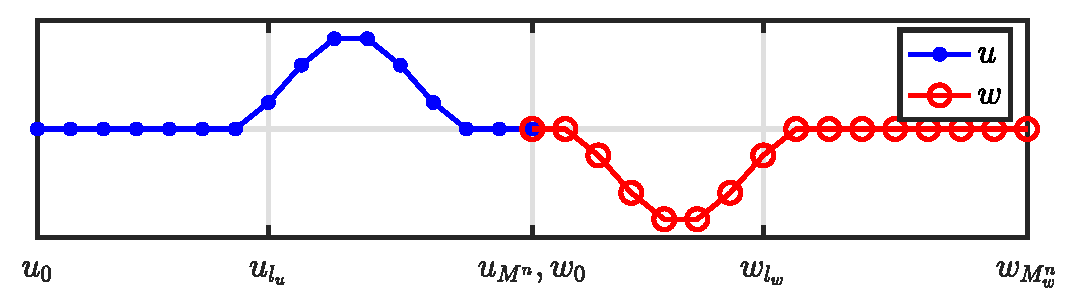
\includegraphics[width=\figwidth\columnwidth]{Figures/twoFreeStringsNarrow.eps}}}\\
    \vspace{-1em}\subfloat[]{\label{fig:twoFreeStringsGridMove}{ 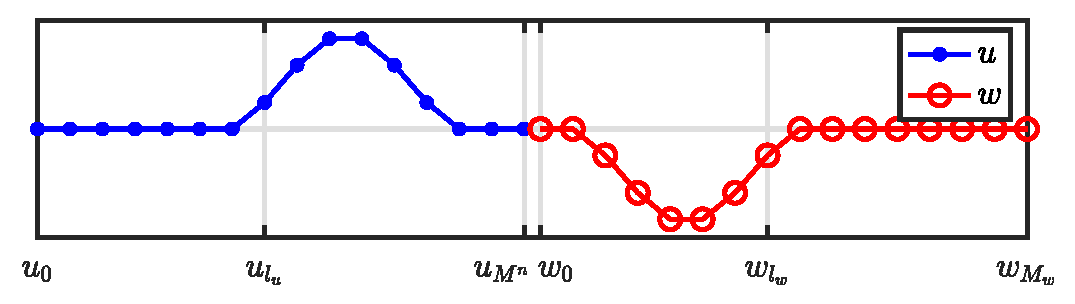
\includegraphics[width=\figwidth\columnwidth]{Figures/twoFreeStringsGridMoveNarrow.eps}}}\\
    \vspace{-1em}\subfloat[]{\label{fig:twoFreeStringsGridZoomed}{ 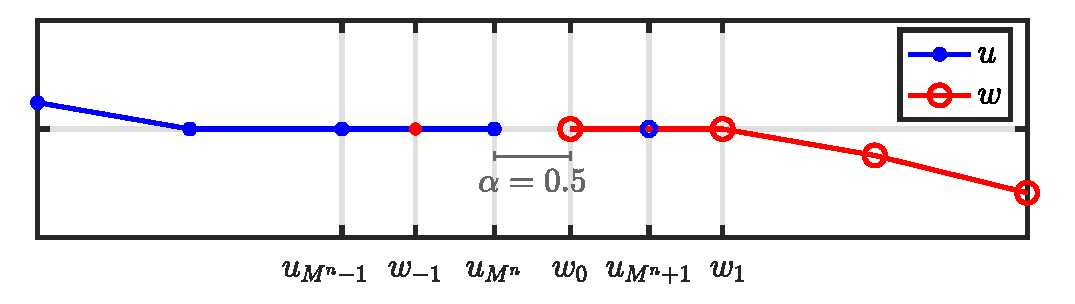
\includegraphics[width=\figwidth\columnwidth]{Figures/twoFreeStringGridMoveZoomedNarrow.eps}}}
    \vspace{-1em}\caption{\it Illustration of the proposed method. In all figures, the x-axis shows the location of the respective grid points%(fx. $x_{u_l^n}$)
    , but `$x^n$' is omitted for brevity. (a) Locations of the states of two (1D wave) systems connected at the inner boundaries ($\Nfrac^n = 30$, $x_{u_{M^n}}^n = x_{w_0}^n$). (b) When $c^n$ -- and consequently $h^n$ -- are decreased and the positions of the grid points change ($\Nfrac^n = 30.5$, $x_{u_{M^n}}^n \neq x_{w_0}^n$). (c) Figure \ref{fig:twoFreeStringsGridMove} zoomed-in around the inner boundaries. The virtual grid points $u_{M^n+1}^n$ and $w_{-1}^n$ are shown together with the distance between them expressed using $\alpha$ in Eq. \eqref{eq:alphaDef}.}
\end{figure}
\SBcomment[OK, in the last panel of Figure 1, the distance between $u_{M}$ and $w_{0}$ looks like a full grid point...but is labelled as $\alpha = 1/2$, which I thought would be a half-grid point distance.] \SWcomment[It is! A gridpoint distance ($h$) is between two blue points or between two red points. This makes the distance between a blue and a red point $0.5h$ or $\alpha = 0.5$. I could make it 0.4 or 0.6 to avoid this confusion..]

\subsubsection{Changing the Grid}\label{sec:changingGrid}
The previous section describes the case in which $\Nfrac^n$ is an integer and condition \eqref{eq:stabilityCond} is satisfied with equality. % $x_{u_M}^n = x_{w_0}^n$. 
We now continue by varying $c^n$ such that this is not the case.

The locations of the outer boundaries $x_{u_0}^n$ and $x_{w_{M_w}}^n$ are fixed:
\begin{equation*}
    x_{u_0}^n = x_{u_0}^0 = 0 \quad \text{and}\quad x_{w_{M_w^n}}^n = x_{w_{M_w^n}}^0 = L \quad \forall n.
\end{equation*}
If the wave speed $c^n$ is then decreased, and consequently the grid spacing $h^n$ according to Eq. \eqref{eq:stabilityCond} (with equality), all other points move towards their respective outer boundary (see Figure \ref{fig:twoFreeStringsGridMove}). Calculating $h^n$ this way allows this method to always satisfy the CFL condition in Eq. \eqref{eq:CFL} with equality, solving issues regarding simulation quality and numerical dispersion described in Section \ref{sec:quality}. %, as is the case with the previous iteration described in \ref{sec:iterations}.

% \begin{figure}[h]
% \centerline{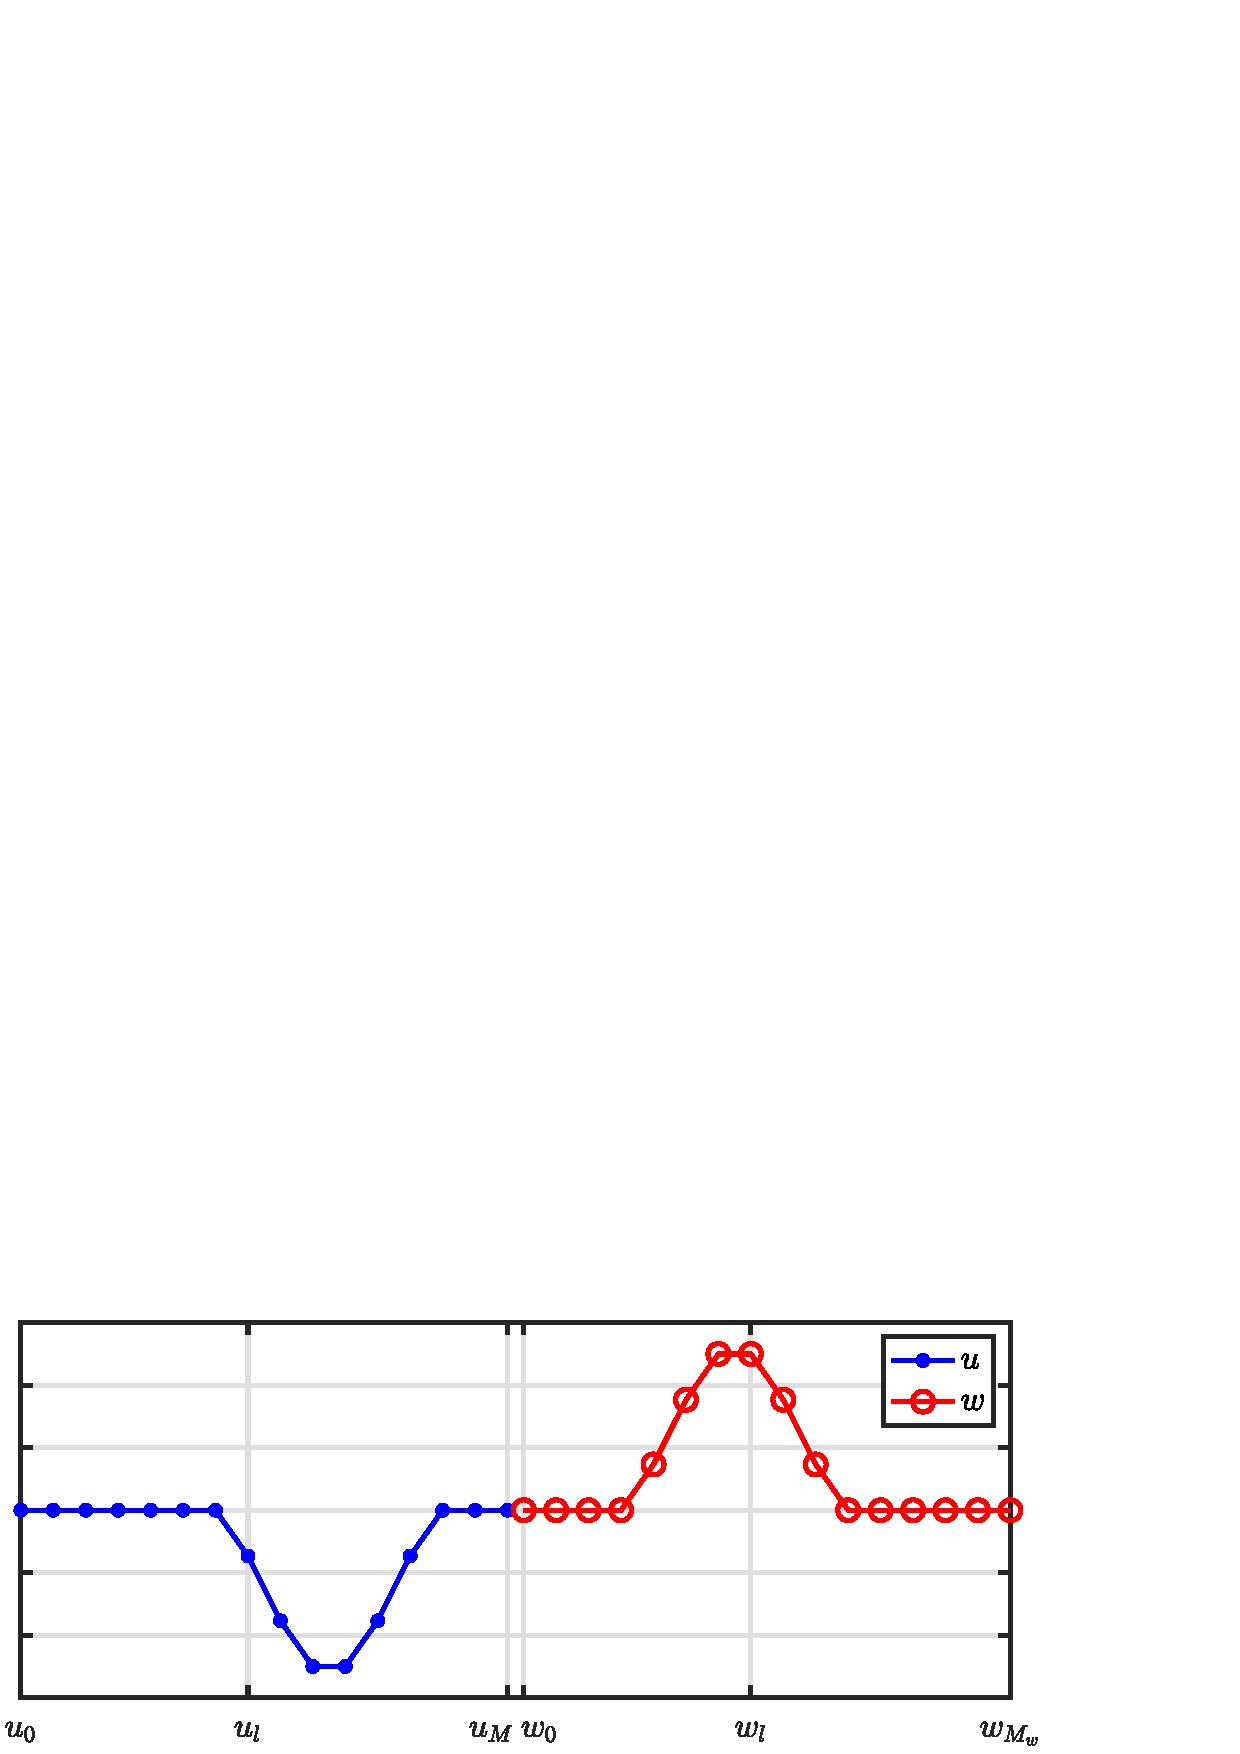
\includegraphics[width=\columnwidth]{twoFreeStringGridMove} }
% \caption{\label{fig:twoFreeStringsGridMove}{When the grid changes ($\Nfrac = 30.5$). The x-axis shows the location (in m) of the respective grid points (fx. $x_{u_l^n}$), but the $x$ is omitted for clarity.}}
% \end{figure}

As mentioned in Section \ref{sec:systSetup}, the state of the virtual grid points at the inner boundaries are defined as $u_{M^n+1}^n = w_1^n$ and $w_{-1}^n = u_{M^n-1}^n$ when the inner boundaries perfectly overlap  (i.e., $x^n_{u_{M^n}} = x^n_{w_0}$). If this is not the case ($x^n_{u_{M^n}} \neq x^n_{w_0}$) a Lagrangian interpolator $I(x_i^n)$ at location $x_i^n$ (in m from the left boundary) can be used to calculate the value of these virtual grid points (also see Figure \ref{fig:twoFreeStringsGridZoomed} for reference). The interpolator $I$ is a row-vector with the same length as $\mathbfcal{U}^n$ (from Eq. \eqref{eq:fullState}) and its values depend on the interpolation order. %Furthermore, the rigid connection in \eqref{eq:rigid} is only valid when the inner boundaries perfectly overlap and does not have to be satisfied when $x_{u_M}^n \neq x_{w_0}^n$. 
In the following, the fractional part of $\Nfrac^n$ %distance between the inner boundaries normalised by $h$ 
is defined as 
\begin{equation}\label{eq:alphaDef}
    \alpha = \alpha^n = \Nfrac^n - N^n %\frac{x^n_{w_0} - x^n_{u_M}}{h}\,,
\end{equation}
\SWcomment[keeping $\alpha$ without superscript for brevity by defining it like this (unless you think for consistency it should have the superscript anyway)] and for clarity, $I$ and $\mathbfcal{U}^n$ are indexed by $m$.
%\SWcomment[it's possible to skip until quadratic interpolation straight away from here, skipping the iterations] In the following, the distance between the inner boundaries normalised with $h$ is defined as
% \begin{equation}\label{eq:alphaDef}
%     \alpha = \alpha^n = \frac{x^n_{w_0} - x^n_{u_M}}{h}\,,
% \end{equation}
% and for clarity, $I$ and $\mathbfcal{U}^n$ are indexed by $m$.
% Applying the interpolator to $\mathbfcal{U}^n$ yields
% \begin{subequations}\label{eq:interpolationGeneral}
%     \begin{align}
%         u_{M+1}^n &= I^\flip(x^n_{u_{M+1}})\mathbfcal{U}^n% = (1-\alpha)w_1^n + \alpha w_0^n
%         \\
%         w_{-1}^n &= I(x^n_{w_{-1}})\mathbfcal{U}^n,% = (1-\alpha)u_{M-1}^n + \alpha u_M^n
%     \end{align}
% \end{subequations}
% where $I^\flip$ is a flipped and shifted version of $I$.
% % where
% % \begin{equation}
% %     \alpha = \frac{x_{w_0} - x_{u_M}}{h},
% % \end{equation}
% % and grid-point locations $x_{u_{M+1}}$ and $w_{-1}$. Note that when $h$ changes the connected points start to move away from each other.
% %
% If linear interpolation is used, 
% \begin{subequations}\label{eq:linearInterp}
% \begin{equation}
%     I_1(x_i) = 
%     \begin{cases}
%         (1-\alpha), & m = m_i \\
%         \alpha, & m = m_i + 1\\
%         0, & \text{otherwise}
%     \end{cases}
% \end{equation}
% and
% \begin{equation}\label{eq:linearFlip}
%     I_1^\flip(x_i) = 
%     \begin{cases}
%         \alpha, & m = m_i^\flip \\
%         (1-\alpha), & m = m_i^\flip + 1\\
%         0 & \text{otherwise}
%     \end{cases}
% \end{equation}
% \end{subequations}
% with $m_i = \lfloor x_i/h\rfloor$ and $m_i^\flip = \lfloor x_i/ h+(1-\alpha) \rfloor$, where the shift in the latter is necessary to transform the location $x_i$ to the right indices of $\mathbfcal{U}^n$. Substituting \eqref{eq:linearInterp} into \eqref{eq:interpolationGeneral} and expanding yields
% \begin{subequations}
%     \begin{align}
%         u_{M+1}^n &= I_1^\flip(x^n_{u_{M+1}})\mathbfcal{U}^n = \alpha w_0^n
%         + (1-\alpha)w_1^n,\\
%         w_{-1}^n &= I_1(x^n_{w_{-1}})\mathbfcal{U}^n = (1-\alpha)u_{M-1}^n + \alpha u_M^n.
%     \end{align}
% \end{subequations}
% % \begin{figure}[h]
% % \centerline{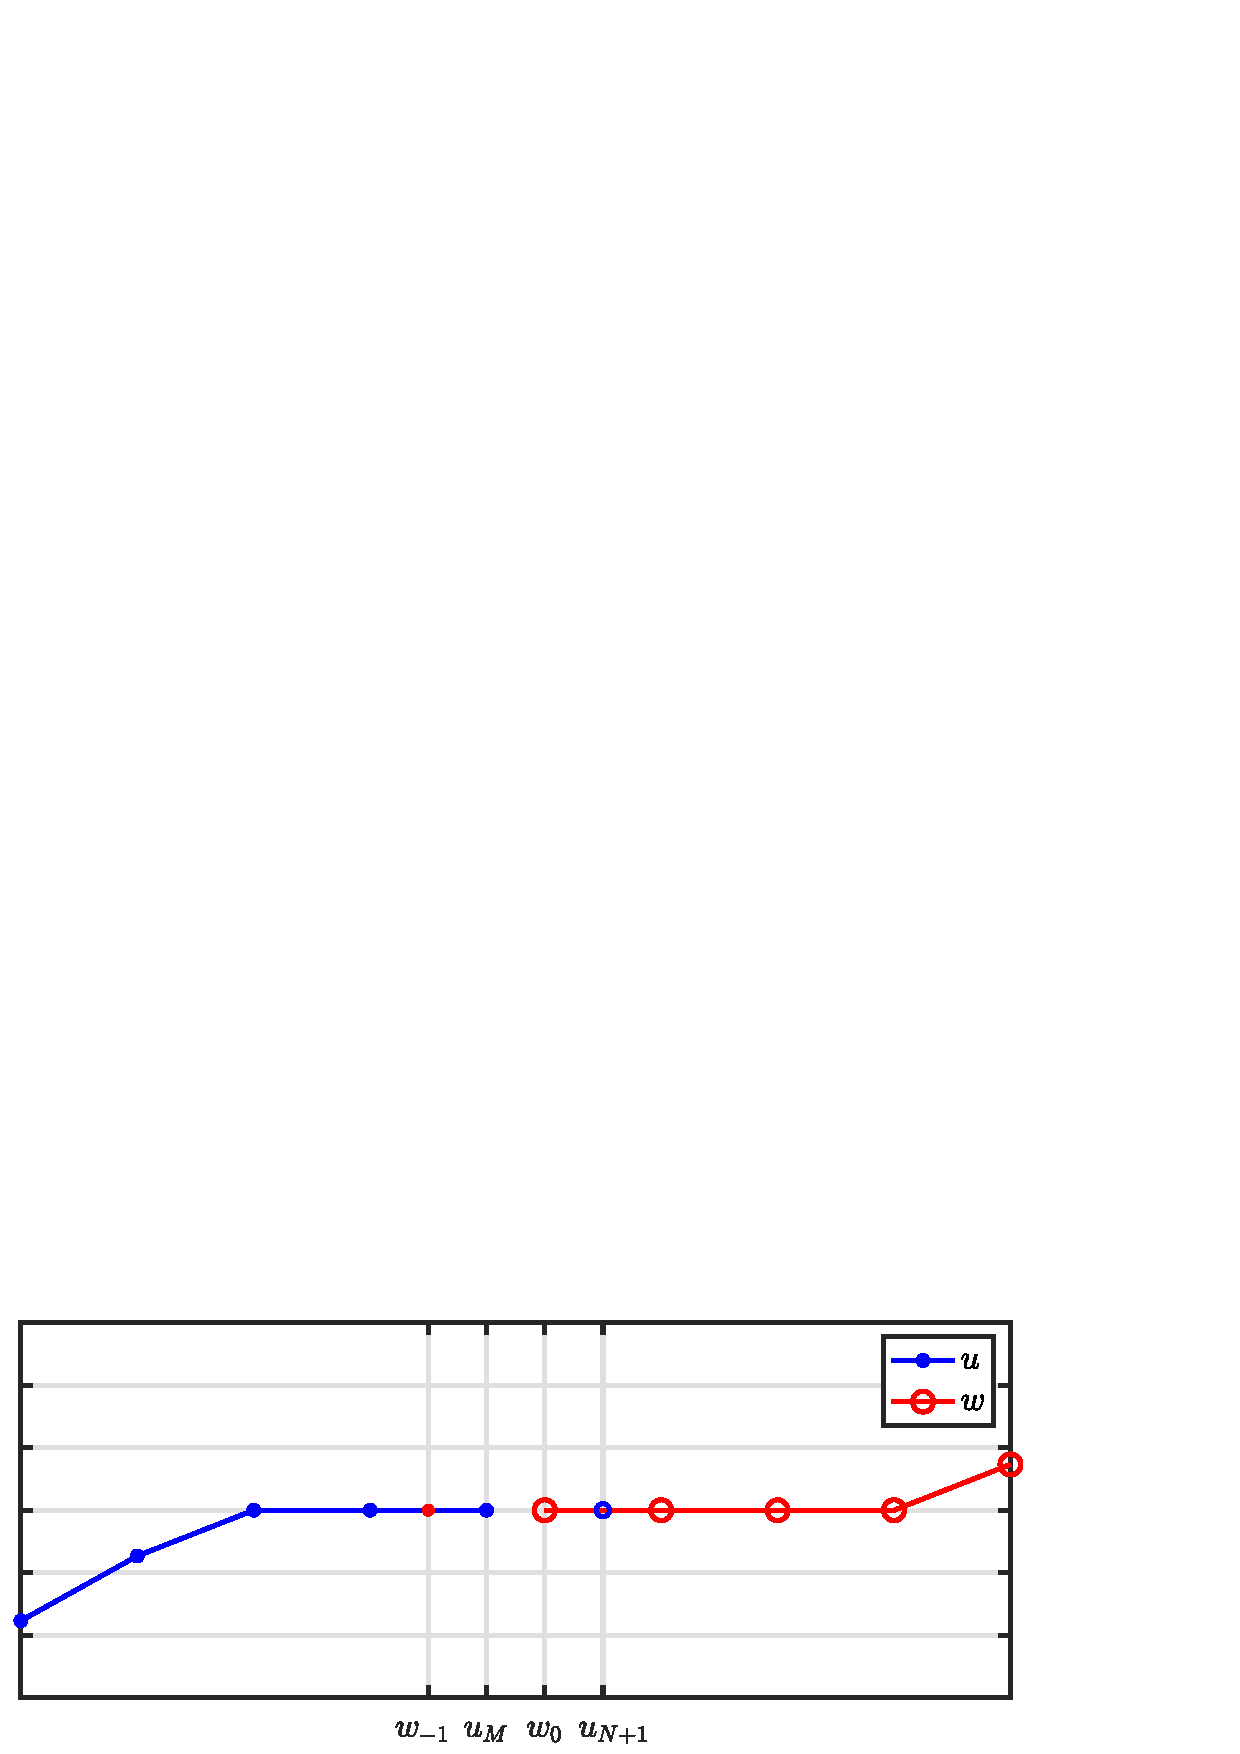
\includegraphics[width=\columnwidth]{twoFreeStringGridMoveZoomed} }
% % \caption{\label{fig:twoFreeStringsGridZoomed}{When the grid changes (zoomed). The states at the inner boundaries $u_M$ and $w_0$ are shown together with virtual grid points $u_{M+1}$ and $w_{-1}$.}}
% % \end{figure}
% %
% Using $I_1$, analysis of the output shows that the expected fundamental frequency $f_0$ is slightly higher when interpolation needs to happen than the one expected when using Eq. \eqref{eq:fundamentalFreq}. Furthermore, modes higher than $f_\text{s} / 4$ would follow an odd pattern up when decreasing the wave speed, opposite of what is expected. \SWcomment[$\leftarrow$ didn't know where (or whether) to include this.]
%
% One could extend the range of interpolation by one point to each side, using a cubic Lagrange interpolator instead. Although this would require $w_{-1}^n$ to calculate $u_{M+1}^n$ and vice versa, it is possible to solve this by treating the interpolation equations as a system of linear equations. Analysis of this method, though yielding a correct $f_0$ at all times, shows similar behaviour to the linear interpolation, with odd behaviour regarding modes higher than $f_\text{s}/4$.
%
% Much better behaviour is observed when points of both $u_l^n$ and $w_l^n$ are used to calculate the values of the virtual grid points. This means to also use $u_M^n$ to calculate $u_{M+1}^n$ and $w_0^n$ for $w_{-1}^n$. Now, the locations of the grid points used in the interpolation are not equidistant and a custom Lagrangian interpolator needs to be created. The lowest order interpolator that can be used here is the quadratic interpolator $I_2$
%
% The best behaviour is observed when $I$ is even-ordered (odd-ordered interpolation results in higher-frequency modes %crossing and
% increasing as $c^n$ decreases and vice-versa) \SBcomment[Could possibly remove this, as it raises a lot of questions...] \MDcomment[I agree ... if you make a comment like this you'd have to give some proof of it.] \SWcomment[Just what is between the parentheses or more..?]. Although higher orders yield slightly better behaviour this improvement is negligible and the lowest even-ordered, quadratic interpolation, already yields good results. The quadratic interpolator $I_2$ is defined as \MDcomment[I would probably just leave out the whole paragraph and just say: "consider the following quadratic interpolator" ]
Now, consider the following quadratic interpolator
\begin{subequations}\label{eq:quadInterp}
\begin{equation}\label{eq:quadNonFlip}
    I_2(x_i^n) =
    \begin{cases}
        -(\alpha-1)/(\alpha + 1), & m = m_i^n-1\\
        1, & m = m_i^n\\
        (\alpha-1)/(\alpha + 1), & m = m_i^n+1\\
        0, & \text{otherwise}
    \end{cases}
\end{equation}
and its flipped version
\begin{equation}\label{eq:quadFlip}
    I_2^\flip(x_i^n) = 
    \begin{cases}
        (\alpha-1)/(\alpha + 1), & m = (m_i^\flip)^n-1\\
        1, & m = (m_i^\flip)^n\\
        -(\alpha-1)/(\alpha + 1), & m = (m_i^\flip)^n+1\\
        0, & \text{otherwise}
    \end{cases}
\end{equation}
\end{subequations}
with $m_i^n = \lfloor x_i^n/h^n\rfloor$ and $(m_i^\flip)^n = \lfloor x_i^n/ h^n+(1-\alpha) \rfloor$ \SWcomment[$m_i$'s also with superscript $n$ here?], where the shift in the latter is necessary to transform the location $x_i^n$ to the right indices of $\mathbfcal{U}^n$.
When applied to Eq. \eqref{eq:fullState} this yields the definitions for the virtual grid points
\begin{subequations}\label{eq:connectionInterpol}
\begin{align}
        &u_{M^n+1}^n = I_2^\flip(x^n_{u_{M^n+1}})\mathbfcal{U}^n = \frac{\alpha - 1}{\alpha + 1}u_{M^n}^n + w_0^n - \frac{\alpha - 1}{\alpha + 1}w_1^n,
    \label{eq:calcUMP1}\\
        &w_{-1}^n = I_2(x^n_{w_{-1}})\mathbfcal{U}^n
        =-\frac{\alpha - 1}{\alpha + 1}u_{M^n-1}^n + u_{M^n}^n+ \frac{\alpha - 1}{\alpha + 1}w_{0}^n.\label{eq:calcWM1}
\end{align}
\end{subequations}
% where
% \begin{equation}\small
% \begin{gathered}\label{eq:interpolationCoeffs}
%     \alpha_\text{I} = \frac{\alpha(\alpha - 1)(\alpha - 2)}{-6}, \quad \beta_\text{I} = \frac{(\alpha - 1)(\alpha + 1)(\alpha - 2)}{2},\\
%     \gamma_\text{I} = \frac{\alpha(\alpha + 1)(\alpha - 2)}{-2}, \quad \text{and} \quad\delta_\text{I} = \frac{\alpha(\alpha + 1)(\alpha - 1)}{6}\,.
% \end{gathered}
% \end{equation}
% Treating \eqref{eq:connectionInterpol} as a system of linear equations, the virtual grid points $u_{M+1}^n$ and $w_{-1}^n$ can be solved for using
% \begin{equation}\label{eq:linSystSolution}
%     \begin{bmatrix}
%     u_{M+1}^n \\
%     w_{-1}^n
%     \end{bmatrix}
%     =
%     \mathbfcal{A}\begin{bmatrix}
%     \alpha_\text{I} w_2^n+ \beta_\text{I}w_1^n + \gamma_\text{I}w_0^n \\
%     \alpha_\text{I} u_{M-2}^n + \beta_\text{I}u_{M-1}^n + \gamma_\text{I} u_{M}^n
%     \end{bmatrix},
% \end{equation}
% where
% \begin{equation}\label{eq:Amat}
%     \mathbfcal{A} = \begin{bmatrix}
%          1 & -\delta_\text{I} \\
%          -\delta_\text{I} & 1
%     \end{bmatrix}^{-1}.\nonumber
% \end{equation}
% where
% \begin{equation}\nonumber
%     \mathbfcal{A} = \begin{bmatrix}
%          1 & -\delta_\text{I} \\
%          -\delta_\text{I} & 1
%     \end{bmatrix},
% \end{equation}
% and
% \begin{equation}\nonumber
%     \mathbf{v} = \begin{bmatrix}
%     \alpha_\text{I} w_2^n+ \beta\text{I}w_1^n + \gamma\text{I}w_0^n \\
%     \alpha_\text{I} u_{M-2}^n + \beta\text{I}u_{M-1}^n + \gamma u_{M}^n
%     \end{bmatrix}.
% \end{equation}
\SWcomment[***$\rightarrow$] These definitions for the virtual grid points at the inner boundaries will replace the Neumann condition in Eq. \eqref{eq:halfStringBoundaryCondNeumann}.\SWcomment[$\leftarrow$***] %As will be shown in Section \ref{sec:results}, quadratic interpolation yields the expected fundamental frequency at all times. 
One can show that when $\Nfrac^n$ is an integer, and thus $\alpha = 0$, Eqs. \eqref{eq:calcUMP1} and \eqref{eq:calcWM1} can be substituted as $w_1^n$ and $u_{M^n-1}^n$ into Eqs. \eqref{eq:resultUM} and \eqref{eq:resultw0} respectively (as these acted as virtual grid points $u_{M^n+1}^n$ and $w_{-1}^n$). Then recalling Eq. \eqref{eq:rigid} it can be seen that the system reduces to \eqref{eq:resultOneConnectedPoint} and exhibits the same exact behaviour as the normal case. % also when interpolation needs to happen.

\SWcomment[***$\rightarrow$]Now that the virtual grid points at the inner boundaries are not determined by the Neumann boundary condition in \eqref{eq:halfStringBoundaryCondNeumann}, but rather by the definitions in Eqs. \eqref{eq:connectionInterpol}, system \eqref{eq:systemHalfStrings} can simply be re-written to
\begin{equation}\label{eq:FDSwithMethod}
    \begin{cases}
        \delta_{tt}u_\lu^n = (c^n)^2\delta_{xx}u_\lu^n\\
        \delta_{tt}w_\lw^n = (c^n)^2\delta_{xx}w_\lw^n
    \end{cases}
\end{equation}
where the Dirichlet condition in \eqref{eq:halfStringBoundaryCondDirichlet} is (still) used for the outer boundaries and the Neumann condition at the inner boundaries in \eqref{eq:halfStringBoundaryCondNeumann} is replaced by the definitions in \eqref{eq:connectionInterpol}
\begin{equation}
        u_{M+1}^n = I_2^\flip(x_{u_{M^n+1}}^n)\mathbfcal{U}^n \quad \text{and}\quad w_{-1}^n = I_2(x_{w_{-1}}^n)\mathbfcal{U}^n.
\end{equation}
\SWcomment[$\leftarrow$***]
% Rewriting system \eqref{eq:systemHalfStrings} to include the method yields 
% \begin{equation}\label{eq:FDSwithMethod}
%     \begin{cases}
%         \delta_{tt}u_\lu^n = (c^n)^2\delta_{xx}u_\lu^n + J_u(x_{u_M}^n)2(c^n)^2\delta_{x\cdot}u_M^n\\
%         \delta_{tt}w_\lw^n = (c^n)^2\delta_{xx}w_\lw^n - J_w(x_{w_0}^n)2(c^n)^2\delta_{x\cdot}w_0^n
%     \end{cases}
% \end{equation}
% where the definitions for the virtual grid points from the second term are defined by the Neumann boundary condition in Eq. \eqref{eq:discreteNeumann} and those from the last terms are found in Eqs. \eqref{eq:connectionInterpol}. \SWcomment[actually it might be better (and more clear) to say that the Neumann condition at the inner boundaries is removed (such that to calculate $u_M^n$ and $w_0^n$ we need $u_{M+1}^n$ and $w_{-1}^n$) and the then-necessary virtual grid points are defined by Eqs. \eqref{eq:connectionInterpol}. Eventually comes down to the same thing... What do you think?]

\subsubsection{Adding and Removing Grid Points}\label{sec:addRemove}
When $c^n$, and consequently $h^n$, are decreased and the inner boundary points surpass the virtual points (i.e. $x_{u_M}^n \leq x_{w_{-1}}^n$ and $x_{w_0}^n \geq x_{u_{M+1}}^n$), which means that $N^n >  N^{n-1}$, a point is added to the right boundary of $u$ and the left boundary of $w$ (for both time indices $n$ and $n-1$) in an alternating fashion: 
\begin{equation}\label{eq:addingPoint}
        \begin{cases}\mathbf{u}^n = [(\mathbf{u}^n)^T, I_3\mathbf{v}^n]^T & \text{if $N^n $ is odd},\\
        \mathbf{w}^n = [I_3^\flip\mathbf{v}^n, (\mathbf{w}^n)^T]^T & \text{if $ N^n$ is even},
        \end{cases}
\end{equation}
where 
\begin{align*}
\mathbf{v}^n = [u_{M-1}^n, u_M^n, w_0^n, w_1^n]^T,% \quad\text{and}\\
%     \mathbf{v}_\star^n &= [w_1^n, w_0^n, u_M^n, u_{M-1}^n],
\end{align*}
and cubic Lagrangian interpolator
\begin{equation}\label{eq:customIp}
    I_3 = \begin{bmatrix} -\frac{\alpha(\alpha+1)}{(\alpha+2)(\alpha+3)} &\frac{2\alpha}{\alpha+2} &\frac{2}{\alpha+2} 
    &-\frac{2\alpha}{(\alpha+3)(\alpha+2)}
    \end{bmatrix},
\end{equation}
with $I_3^\flip$ being just a flipped, not shifted, version of \eqref{eq:customIp}.
%with
% \begin{equation*}
%     \alpha' = \frac{x_{w_0}^n - (x_{u_M}^n + h)}{h}\ .
% \end{equation*}
See Figure \ref{fig:addingPoint}.
% Note that this operation is done for both time indices $n$ and $n-1$.
%
\begin{figure}[t]
    \centering
%% \reprintcolumnwidth is the same in preprint and reprint for
%% ease of use for authors:
\includegraphics[width=\figwidth\columnwidth]{Figures/addingGridPointNarrow.eps}
\caption{\label{fig:addingPoint}{\it The moment when a point is added to $\mathbf{u}$ at location $x_{u_{M^n}} + h$ in Eq. \eqref{eq:addingPoint}. This figure shows an extreme case where this location is far from $x_{w_0}$, i.e., $\alpha \not\approx 0$ in Eq. \eqref{eq:customIp}.}}
\end{figure}
Notice that $\Nfrac^n$ is only going to be slightly bigger than an integer at the moment that a point is added (except in the case of extremely quick parameter variations) and Eq. \eqref{eq:alphaDef} will return $\alpha \gtrsim 0$.
%\MDcomment[Okay, I don't quite get this ... why cannot $\alpha$ be close to 1 here? In fact, it will be close to 1 when a point is about to be created ... I don't understand how the rate of change of $c$ affects the value of $\alpha$] \SWcomment[Right when a point is supposed to be added, $N^n$ is going to be slightly bigger than an integer value. Just to clarify, $N^n$ is first retrieved and then used to calculate $\alpha$ in \eqref{eq:alphaDef}. In quick parameter variations $N^{n-1}$ might be fx. 0.99, and $N^{n}$ fx. 0.3. Then $\alpha \not\gtrsim 0$. The way that the rate of change of $c$ is linked to $\alpha$ is that there is only $1/f_\text{s}$ seconds difference between $n$ and $n-1$.]
% ,  $\alpha$ in Eq. \eqref{eq:customIp} is expected to be close to zero, %, i.e., $x_{u_M}^n + h \approx x_{w_0}^n$,
This means that that $I_3 \approx [0, 0, 1, 0]$ and the displacement of the newly added point is nearly fully based on the grid point at the inner boundary of the other system. %This makes sense by looking at Figure \ref{fig:twoFreeStringsGridZoomed}, as exactly when the boundary points $u_M^n$ and $w_0^n$ surpass the virtual points $w_{-1}^n$ and $u_{M+1}^n$, these are going to be close to overlapping.

Removing grid points happens when $c^n$, and consequently $h^n$, are increased and $x_{u_M}^n \geq x_{w_0}^n$ (or $ N^n <  N^{n-1}$). %Compared to adding grid points, removing these is slightly more straightforward as points 
Grid points are simply removed from $\mathbf{u}$ and $\mathbf{w}$ (again for both $n$ and $n-1$) in an alternating fashion according to
\begin{equation}\label{eq:removingPoint}
\begin{cases}
    \mathbf{u}^n = [u_0^n, u_1^n ..., u_{M^n-1}^n]^T & \text{if $N^n$ is even}, \\
     \mathbf{w}^n = [w_1^n, w_2^n ..., w_{M_w^n}^n]^T & \text{if $N^n$ is odd}.
    \end{cases}
\end{equation}
In Eqs. \eqref{eq:addingPoint} and \eqref{eq:removingPoint}, the even and odd conditions can be inverted. To keep the difference between $u$ and $w$ a maximum of one grid point, the ceiling and flooring operations when calculating $M^n$ and $M_w^n$ will need to be inverted as well.

Until now, only adding and removing points in the center of the original system has been considered. This location could be moved anywhere along the grid, the limit being one point from the boundary. In other words, both $u_\lu^n$ and $w_\lw^n$ need to have at least one point (excluding the grid functions at the outer boundaries). Furthermore, one does not have to add and remove points from $\mathbf{u}$ and $\mathbf{w}$ in an alternating fashion as in \eqref{eq:addingPoint}, but can just add and remove from (fx.) $\mathbf{u}$ leaving $\mathbf{w}$ the same size throughout the simulation. In the extreme case where $M^n = N^n - 1$ and $M_w^n = 1$ (leaving $w_\lw^n$ with only one moving grid point, $w_0^n$) the method still works.

\subsubsection{Displacement correction}\label{sec:dispCorr}
A problem that arises when increasing $c^n$, is that it is possible that the displacements $u_M^n \not\approx w_0^n$ at the time when a grid point needs to be removed. As the grid locations $x_{u_M}^n \approx x_{w_0}^n$ at the time of removal (except for extremely quick parameter variations), this violates the rigid connection in \eqref{eq:rigid} and causes audible artefacts. A method is proposed that decreases the relative displacement of the inner boundaries the closer their grid-locations are together, i.e., the closer $\alpha$ in \eqref{eq:alphaDef} is to 0. We thus extend system \eqref{eq:FDSwithMethod} with an artificial spring force as
\begin{equation}\label{eq:sysDispCorr}
\begin{cases}
    \delta_{tt}u_\lu^n = (c^n)^2\delta_{xx}u_\lu^n+ J_u(x_{u_M}^n)%\left(2(c^n)^2\delta_{x\cdot}u_M^n + F_\text{c}^n\right)
    F_\text{c}^n,\\
    \delta_{tt}w_\lw^n = (c^n)^2\delta_{xx}w_\lw^n - J_w(x_{w_0}^n)%\left(2(c^n)^2\delta_{x\cdot}w_0^n+F_\text{c}^n\right)
    F_\text{c}^n.
\end{cases}
\end{equation}
Using centred temporal averaging and difference operators
\begin{subequations}\label{eq:centredOperators}
\begin{align}\label{eq:centredAverage}
    \mu_{t\cdot}\ugen_l^n &= \frac{1}{2} \left(\ugen_l^{n+1} + \ugen_l^{n-1}\right),\\
    \delta_{t\cdot}\ugen_l^n &= \frac{1}{2k} \left(\ugen_l^{n+1} - \ugen_l^{n-1}\right),
\end{align}
\end{subequations}
the correction effect %(in m$^2/$s$^2$) 
is defined as %\SWcomment[something off with the units here. I think I took this from the scaled version and assumed that $J$ has units of m$^{-1}$ (due to $1/h$).] is modelled as a spring-like connection and is defined as
\begin{equation}\label{eq:dispCorrForce}
    F_\text{c}^n = \beta \left(\mu_{t\cdot}\eta^n +\sigma_0\delta_{t\cdot}\eta^n \right).
\end{equation}
%\MDcomment[It seems that $\omega_0$ is somewhat redundant here.] \SWcomment[Actually, I did that for the units to add up (didn't have it before, as it is only the ratio between $\omega_0^2$ and $\sigma_0$ that matters..). As I plan to take away the units (since it's an arbitrary connection) should I remove it you think?] \MDcomment[Also, why multiply $\sigma_0$ by $\beta$? ... not very clear.] \SWcomment[$\beta$ simply scales the entire correction effect. Apart from force, I don't want there to be much damping effect when $\alpha$ is not close to 0 either.] 
with the difference in displacement between the inner boundaries
\begin{equation}\label{eq:etaDispCorr}
    \eta^n \triangleq w_0^n - u_M^n,
\end{equation}
and damping coefficient $\sigma_0$% (in s$^{-1}$)
. Furthermore, $\beta$ scales the effect of the displacement correction and is defined as
\begin{equation}\label{eq:betaDef}
    \beta = \beta(\alpha) = \frac{1-\alpha}{\alpha + \varepsilon}\ ,
\end{equation}
%(in m) \SWcomment[for the units to make sense... I guess it includes the $1/\rho A$ (for a 1D wave modelling a string without stiffness) but as it is an artificial connection force, it might make more sense to exclude all units here..] 
where $\varepsilon \ll 1$ prevents a division by 0. Despite the operators in \eqref{eq:centredOperators} introducing states at $n+1$, it is possible to calculate the force explicitly (such as in \cite{bilbao2009} or \cite{bilbao2009Dafx}). Furthermore, it can be shown that even when $\varepsilon = 0$ this calculation is always defined. In that case, as $\alpha \rightarrow 0$, $\beta\rightarrow \infty$ 
%\MDcomment[I don't quite get this. Why do you need to divide by $\alpha$ in (35)?] \SWcomment[To get $\beta \rightarrow \infty$ as $\alpha \rightarrow 0$ :)] \MDcomment[Also how is $\varepsilon$ chosen?] \SWcomment[It is set to 0 in the implementation. Do you think I should exclude it and just elaborate on the fact that even when $\beta \rightarrow \infty$ the calculation is defined?] \MDcomment[And how is the connection rigid when $\alpha = 0$?  Shouldn't a rigid connection have $\beta \rightarrow \infty$ ] \SWcomment[but it does! As I say, when $\epsilon = 0$ and $\alpha = 0$, $\beta\rightarrow \infty$. $\beta$ is simply a function that goes ("asymptotically") from $0$ to $\infty$ as $\alpha$ goes from $1$ to $0$] 
which acts as a rigid connection such as Eq. \eqref{eq:rigid}. Essentially, the displacement correction attempts to have $\eta^n\rightarrow 0$ in Eq. \eqref{eq:etaDispCorr} as $\alpha \rightarrow 0$ to satisfy the rigid connection in Eq. \eqref{eq:rigid}.
Although the correction presented here is not based on some physical process, it could be justified by the fact that large differences in displacement between two spatially adjacent points is not physical. \SWcomment[$\leftarrow$ tried to justify]

Notice that when $c^n$ is decreased, the rigid connection will not be violated as $u_M^n \approx w_0^n$ when a point is added. This is due to the fact that $I_3\approx [0, 0, 1, 0]$ and either $u_M^n$ or $w_0^n$ is the newly added point which almost solely based on the other (for low-speed parameter variations).
% \MDcomment[I have the feeling that this whole subsection is not very clear ... reviewers might jump on this, because there is no real justification for this extra spring system in here, outside of the fact that you hear artefacts and try to make up for it by adding this in. ] \SWcomment[I tried to justify at the beginning of \ref{sec:dispCorr} that differences in displacements while $\alpha \gtrsim 0$ violate the rigid connection and that this is a way to smoothly go towards this when increasing $c^n$. But I can see that this might not be enough. What do you propose? :)] \MDcomment[I don't know, it just looks strange that you need to do this. In fact, it's strange that you need two grids! Why not just work with one grid, where you fit the right boundary so to take into account the fractional grid spacing? Having two grids connected at the centre just sounds like a bit of a mess ...] \SWcomment[AHH entire method gone hahaha. No, been there, done that, unfortunately (as far as I know...). You can't do the quadratic interpolation then as you have too few points and you'll get weird behaviour with linear interpolation (as you might remember: modal crossings, opposite moving modal frequencies above $0.25 f_\text{s}$). And even there you'll need to "guide" the displacement of the grid point you're about to remove to the boundary value (which is 0 for Dirichlet) when decreasing $N$ as they will still have some "moment" or "inertia" from the $\delta_{tt}u$ term. In other words, right before removing a grid point, it will still be moving if it had earlier in the simulation, consequently, the Dirichlet boundary term will be violated, similar to how the rigid connection is violated here.\\
% One moving point with the proposed method is as close to adding / removing at the boundary as you'll get (as I describe in Section \ref{sec:addRemove}) and with a large system, this is basically the same as doing it at the boundary ;) I hope this all makes sense..]
% \MDcomment[It's just really strange that you are saying that (17) is valid $\forall$ n, when in fact in Fig 1 the points are far apart ... and here in 4.1.4 you are in fact saying that these points are not going to be equal. What is the point of introducing (17) then if you are going to have them connected with a spring? It seems that (17) is never really implemented ...
% Also, what is the purpose of the loss in the spring?] \SWcomment[You're right about the $\forall n$ in \eqref{eq:rigid}, I changed that and added to the condition that the rigid connection only holds when the inner boundaries perfectly overlap ($\alpha = 0$). The damping is so that you don't get highly oscillatory behaviour when $\alpha \gtrsim 0$. At least, that is what I observed. The damping lets the grid points at the inner boundaries go closer and closer together (more and more satisfying the rigid connection).]
% \MDcomment[It just looks not very well justified. There is not real ground to make these claims ... something reviewers will certainly notice!] \SWcomment[I'll try to justify it a bit more. Thanks!]
%$\beta$ can be seen as a spring force pulling the inner boundaries to the average displacement between them. A lower $\varepsilon$ decreases the chance of artifacts but will have a greater filtering effect on the system. For low-speed changes, using $\sim 1000$ samples for removing one grid point, $\varepsilon \approx 30$ ensures that $u_M^n \approx w_0^n$ at the time of removal and already suffices to remove artefacts.

% 
% \SWcomment[The following applies to odd-ordered Lagrange interpolators $\rightarrow$] The location at where points are added and removed greatly influences the behaviour of the system, especially in the higher frequencies (see Section \ref{sec:results}). The best behaviour is obtained when the location is as close to a boundary as possible. 

\subsection{Summary}
Here, Section \ref{sec:proposedMethod} is summarised and describes the final version of the proposed method.

The proposed method subdivides a grid function $\ugen_l^n$ with $N$ intervals into two grid functions $u_\lu^n$ and $w_\lw^n$ with $M^n$ and $M_w^n$ intervals respectively for a total of $N^n+2$ grid points. Knowing that $\lambda=1 \ \forall n$, Eq. \eqref{eq:updateEq}, written for both grid functions, becomes 
\begin{subequations}\label{eq:uwUpdates}
    \begin{align}
        u_\lu^{n+1} &= u_{\lu+1}^n + u_{\lu-1}^n - u_\lu^{n-1},\label{eq:uUpdate}\\
        w_\lw^{n+1} &= w_{\lw+1}^n + w_{\lw-1}^n - w_\lw^{n-1}\label{eq:wUpdate}.
    \end{align}
\end{subequations}
%
Due to the Dirichlet boundary condition in \eqref{eq:halfStringBoundaryCondDirichlet} imposed at the outer boundaries of the system, $u_0^n$ and $w_{M_w}^n$ are $0$ at all times and do not have to be included in the calculation. The ranges of calculation for Eq. \eqref{eq:uUpdate} and \eqref{eq:wUpdate} then become $\lu \in \{1, \hdots, M^n\}$ and $\lw \in \{0, \hdots, M_w^n - 1\}$ respectively. 

The grid points at the inner boundaries are calculated by expanding \eqref{eq:FDSwithMethod} (ignoring the displacement correction for now)
\begin{subequations}\label{eq:innerboundariesExpanded}
    \begin{align}
        u_M^{n+1} &= u_{M+1}^n + u_{M-1}^n - u_M^{n-1},\\
        w_0^{n+1} &= w_{-1}^n + w_{1}^n - w_0^{n-1}.
    \end{align}
\end{subequations}
%
where virtual grid points $u_{M+1}^n$ and $w_{-1}^n$ can be calculated using Eq. \eqref{eq:connectionInterpol}.

Then, when $ N^n > N^{n-1}$ a point is added to $\mathbf{u}^n$ and $\mathbf{u}^{n-1}$ (or $\mathbf{w}^n$ and $\mathbf{w}^{n-1}$) using Eq. \eqref{eq:addingPoint}, and when $ N^n  < N^{n-1}$ a point is removed from the same vectors using Eq. \eqref{eq:removingPoint}. In order to prevent audible artefacts when increasing $c^n$ (and thus decreasing $\Nfrac^n$) due to a violation of the rigid connection in \eqref{eq:rigid}, a method in \eqref{eq:sysDispCorr} is proposed to ensure that the grid points at the inner boundaries have a similar displacement when one of them is removed. 

% \MDcomment[I think it would be a lot cleaner if you wrote down the form of $Dxx$ and therefore gave a FD equivalent of (1). For the same reason, it would be better to stick to $\bf q$ for notation. So, you could have $\delta_{tt} {\bf Q}^n = c^n {\bf D}_{xx}{\bf Q}^n$] \SWcomment[Hmm.. but $\mathbf{D}_{xx}$ does not work here due to all the additional stuff (interpolation, displacement correction) right?] \MDcomment[You can definitely define a Dxx operator that includes all that, depending on alpha, beta, etc] \SWcomment[Actually, now that I don't do the modal analysis stuff in detail anymore I can just remove the matrixforms here (will also save some space) $\rightarrow$]
% Finally, using $\mathbfcal{U}$ from Eq. \eqref{eq:fullState} the total system can be compactly written in matrix form as
% \begin{equation}\label{eq:totalSystem}
%     \mathbf{C}_+^n\mathbfcal{U}^{n+1} = 
%     \mathbf{B}^n
%     \mathbfcal{U}^n
%     + \mathbf{C}_-^n\mathbfcal{U}^{n-1}
% \end{equation}
% with $ N^n \times N^n$ matrices
% \begin{equation}\label{eq:bMat}
%     \mathbf{B}^n = 
%     % \begingroup % keep the change local
%     % \setlength\arraycolsep{2pt}
%     \begin{bmatrix}[cccc|cccc]
%         & \ddots  &\ddots & & & & 0 & \\
%           & 1 & 0 & 1 & & & & \\
%          & & 1 & \frac{\alpha - 1}{\alpha + 1} & 1  & -\frac{\alpha - 1}{\alpha + 1} & \\ \cline{2-7}
%          & & -\frac{\alpha - 1}{\alpha + 1} & 1  & \frac{\alpha - 1}{\alpha + 1}  & 1 & & \\
%             & & & &1 & 0 & 1  \\
%             & 0 & &  &  &\ddots & \ddots &
%       \end{bmatrix}
%     %    \endgroup
% \end{equation}
% containing the effect of the general method described in Section \ref{sec:changingGrid} and
% \begin{equation}\label{eq:CMat}
%     \mathbf{C}_\pm^n = \pm\left(\mathbf{I}^n - \frac{\beta k^2 (\omega_0^2\pm\sigma_0/k)}{2}\mathbf{J}^n\boldsymbol{\eta}^n\right)
% \end{equation}
% containing the effect of the displacement correction described in Section \ref{sec:dispCorr} where $\mathbf{I}$ is the $ N^n \times N^n$ identity matrix and 
% \begin{equation}
%     \mathbf{J}^n = [\mathbf{0}_{M^n-1}, 1/h^n, -1/h^n, \mathbf{0}_{M_w^n-1}]^T
% \end{equation}
% and 
% \begin{equation}
%     \boldsymbol{\eta}^n = [\mathbf{0}_{M^n-1}, -1, 1, \mathbf{0}_{M_w^n-1}]
% \end{equation}
% are vectors of length $N^n$ and $\boldsymbol{0}_i$ is a zero-vector of length $i$.
%
% \begin{equation}\small
%     \mathbf{B} = \begin{bmatrix}[ccccccc|cc]
%     & &\ddots &\ddots & \ddots  & & \mathbf{0} & & \\
%      & & &1 & 0 & 1 & & \mathbf{0} & \\
%      & & &  & 1 & 0 & 1 & & \\
%      & &\mathbf{0} &  & \mathbfcal{A}_{1, 2}\alpha_\text{I} &\mathbfcal{A}_{1, 2}\beta_\text{I} + 1 &\mathbfcal{A}_{1, 2}\gamma_\text{I} & \mathbfcal{A}_{1, 1}(\gamma_\text{I}-\alpha_\text{I})& \\ \cline{2-8}
%      & & \mathbf{0} & &\mathbfcal{A}_{2, 2}\alpha_\text{I} &\mathbfcal{A}_{2, 2}\beta_\text{I}&\mathbfcal{A}_{2, 2}\gamma_\text{I} & \mathbfcal{A}_{2,1}(\gamma_\text{I} - \alpha_\text{I}) & 
%     \end{bmatrix}
% \end{equation}
%
% Notice that as $\alpha$ approaches $1$, $\mathbf{B}$ reduces to a matrix with ones on the diagonals next to the main diagonal and zeros elsewhere, which translates directly to the normal case in Eq. \eqref{eq:updateEq} with $\Nfrac^n = M^n + M_w^n + 1$. 

\subsection{Implementation}
A MATLAB implementation of the proposed method can be found via \cite{MATLABcode} and Algorithm \ref{alg:calcOrder} shows the order of calculation of this implementation. Especially important to take into account, is to only retrieve a change in $c^n$ at time index $n$ once before all other calculations. This is to ensure that $u_\lu^n$ and $w_\lw^n$ are calculated with the same $\alpha$ and $\beta$ for all $\lu$ and $\lw$.
\begin{algorithm}[ht]
    \setstretch{1.1}
    \fbox{\parbox{0.8\linewidth}
    {
        \While{application is running}
        {
            \begin{minipage}[c]{0.9\linewidth}
                Retrieve new $c^n$\\
                Calc. $h^n$ (Eq. \eqref{eq:stabilityCond} with equality)\\
                Calc. $\Nfrac^n$ and $N^n$ (Eqs. \eqref{eq:fundamentalFreq} and \eqref{eq:orderOfCalcGrid}) \\
                Calc. $\alpha$ (Eq. \eqref{eq:alphaDef})\\
                \If{$ N^n \neq N^{n-1} $}
                {
                    Add or remove point (Eq. \eqref{eq:addingPoint} or \eqref{eq:removingPoint})\\
                    Update $M^n$ and $M_w^n$
                }
                % \If{$\lfloor N^n\rfloor > \lfloor N^{n-1} \rfloor$}
                % {
                %     Add point (Eq. \eqref{eq:addingPoint})\\
                %     Update $M$ and $M_w$
                % }
                % \ElseIf{$\lfloor N^n\rfloor < \lfloor N^{n-1} \rfloor$}
                % {
                %     Remove point (Eq. \eqref{eq:removingPoint})\\
                %     Update $M$ and $M_w$
                % }
                % Calc. $\beta$ (Eq. \eqref{eq:betaDef})\\
                % Update $\mathbf{B}$ and $\mathbf{C}_\pm$ (Eqs. \eqref{eq:bMat} and \eqref{eq:CMat})\\
                % Calc. scheme (Eq. \eqref{eq:totalSystem})\\
                Calc. $u_\lu^{n+1}$ and $w_\lw^{n+1}$ (Eqs. \eqref{eq:uwUpdates} and \eqref{eq:innerboundariesExpanded})\\
                Calc. and apply displacement corr. (Eq. \eqref{eq:dispCorrForce})\\
                Retrieve output\\
                Update states ($\U^{n-1} = \U^n$, $\U^n = \U^{n+1}$)\\
                Update $N^{n-1}$ ($N^{n-1} = N^n$)\\
                Increment $n$
            \end{minipage} 
            % \begin{minipage}[c]{0.4\linewidth}
            % -\\
            % \vspace{2em}(Eq. \eqref{eq:addingPoint})\\
            
            % (Eq. \eqref{eq:removingPoint})\\

            % \end{minipage}
            }
        }
    }
    \vspace{0.12cm}
    \caption{\it Pseudocode showing the order of calculations.\label{alg:calcOrder}}
\end{algorithm}